\documentclass[a4paper, english, 12pt]{scrartcl}
\usepackage[utf8]{inputenc}
\usepackage[T1]{fontenc}
%\usepackage{babel}
\usepackage{graphicx}
\usepackage{subfigure}
\usepackage[amssymb,binary]{SIunits}
\usepackage{amsmath,amsfonts,amssymb,textcomp,varioref}
\usepackage{listings}
\usepackage{times}
\usepackage{nomencl}


%\usepackage[margin=2cm]{geometry}

%\setlength{\parindent}{0 pt}
%\addtolength{\parskip}{\baselineskip}
%\usepackage{setspace}
%\doublespacing

\usepackage{hyperref}

\renewcommand{\nomname}{List of Abbreviations}
\makenomenclature


\lstset{ %
basicstyle=\footnotesize,       % the size of the fonts that are used for the code
numbers=left,                   % where to put the line-numbers
numberstyle=\footnotesize,      % the size of the fonts that are used for the line-numbers
stepnumber=1,                   % the step between two line-numbers. If it's 1 each line will be numbered
numbersep=5pt,                  % how far the line-numbers are from the code
showspaces=false,               % show spaces adding particular underscores
showstringspaces=false,         % underline spaces within strings
showtabs=false,                 % show tabs within strings adding particular underscores
frame=single,                % adds a frame around the code
tabsize=3,                % sets default tabsize to 2 spaces
captionpos=b,                   % sets the caption-position to bottom
breaklines=true,                % sets automatic line breaking
breakatwhitespace=false,        % sets if automatic breaks should only happen at whitespace
escapeinside={\%*}{*)}          % if you want to add a comment within your code
}


% Set the beginning of a LaTeX document
\begin{document}

\title{Clockless AES circuit}
\author{Kristoffer Ellersgaard Koch}

\date{Fall 2009}
\pagenumbering{roman} % i, ii, iii, iv...
\pagestyle{empty}
\maketitle
\thispagestyle{empty}

\cleardoublepage
\pagestyle{plain}
\thispagestyle{plain}
\section*{Assignment description}

Challenging the frontiers of ultra low-energy design requires
innovative low-energy contributions from all levels and aspects of the
design and toolflow. Software architecture, digital system-level
architecture, low-level digital design choices, backend techniques
such as clock gating strategies, toggle information feedback and
operand isolation, process technology and place-and-route techniques
are all critical factors in the total digital world energy consumption
budget.

Some fundamental paradigms of main-stream digital design flows have
not changed for decades, such as the presence of a clock. Research
into self-timed techniques (we are avoiding the term ‘asynchronous’
here because an asynchronous design often refers to a design with
multiple asynchronous clocks) has progressed steadily over the last
two decades. Self-timed design promises major improvements in energy
consumption and noise emission compared to traditional clocked
synchronous designs.

A major hurdle that had to be solved to enable large scale
commercialized of such circuits was testability. Until recently,
self-timed digital circuits were not scanable, and therefore
traditional production testing and low-cost mass production was not
possible.

A range of different approaches have been developed for the design and
synthesis of self-timed circuits. The Netherlands based company
Handshake Solutions (www.handshakesolutions.com) is one example of a
tool and IP provider for self-timed circuit design.

The focus of this thesis is to conduct a pre-study into the viability
of using self-timed design techniques for low-cost ultra-low energy
designs such as the EFM32 microcontroller family. Such techniques will
not be applicable for the entire digital part of a MCU, but for
certain peripheral and core modules. In this thesis, a study into
converting a synchronous Advanced Encryption Standard (AES) peripheral
module into a self-timed and scanable peripheral module is the primary
objective. Various self-timed techniques should be explored and
compared to a traditional synchronous design.

\newpage
\pagestyle{plain}
\thispagestyle{plain}
\section*{Abstract}

Design of digital circuits usually involves a clock. The clock can
however, be one of the greatest contributers to power consumption, and
it is increasingly difficult to distribute a clock over a large
circuit. There exists work on clockless design, and instead use
self-timed techinques to replace the clock. However, theese techniques
are not widely known.

In this project, design of clockless circuits was explored by a
litterature study, and implementation of a clockless Advanced
Encryption Standard (AES) to show the feasability of implementing
reasonable complex clockless circuits. Methods for production testing
were also found.

The result of the study yielded a large AES-module, suggestions for a
workflow for implementing clockless circuits, and pointers to further
research on clockless circuits.

\newpage

\tableofcontents
\listoffigures

\printnomenclature
\newpage
\setcounter{page}{1}
\pagenumbering{arabic} % 1, 2, 3...
\section{Introduction}

One major assumption in the majority of digital VLSI circuits produced
today, is the notion of a discrete and common time. This is provided
by one or more clocks. This is an important simplification that makes
reasoning about digital circuits easyer. However, as circuits grow in
size and complexity, the task of providing a clock-signal
simultaneously to all flip-flops in the circuit becomes an
increasingly difficult task.

When designing a digital circuit for solving a computable problem, it
is usual to split the problem into multiple combinatorical circuits
with memory elements between them. The value of a memory element is
then determined by the value of the previous memory element modified
by a combinatorical circuit. However, this combinatorical circuit has
a non-zero delay, and there is usually no reliable way to assure that
the output value has been completly calculated. With clocked circuits,
the completeness of a calculation is guaranteed by assuming worst case
conditions and setting the clock-frequency accordingly.

As digital circuits have grown, designing has decreasingly become a
problem of specification, and increasingly become problem of managing
complexity. Hardware description languages, such as VHDL and Verilog,
is maybe the most important tools to manage complexity for digital
designers.

In this project, I will investigate options for synthesizing digital
circuits without clocks. A prerequisite for such solutions is a
high-level language that ultimatly can be implemented in silicon. I
will also attempt to implement an encryption-circuit for the
AES-standard with one of theese technologies.

The motivation for investigating clockless is that the clock, while
conceptually simple, imposes increased complexity when the circuits
grow; the clock can ultimatly end up complicating the design instead
of simplifying it. Modern CAD tools employ complex and proprietary
techniques for distributing the clock througout the circuit.

Clockless circuits also have different and interesting characteristics:
\begin{itemize}
\item The clock in a conventional design is one of the main contributer to
power-consumption. 

\item The simultanity of the clock make the circuits exhibit noticeable
spikes in the electromagnetic spectrum.

\item The whole problem of clock domain crossing is sidestepped, allowing a
higher degree of modularity and reuseability.

\item Clockless designs are more robust to process techonlogies and
operating conditions. Clockless circuits operates at its highest
possible speed, and adapts to doping variations, bending and stretching in
contemporary strechable circuits, temperature and voltage.

\item Clockless circuits does not require massive, ``cheap'', metallic
fan-outs provided by the silicon-techonlogy today. Future technologies
for implementing logic, such as ``rapid single flux quantum'', does not
provide a similar simple fan-out mechanism. 
\end{itemize}

When mapping high-level description hardware-languages to silicon,
there must also be implemented a form of completion-detection for the
combinatorical circuits to drive the memory-elements instead of the
clock. I will outline multiple of these techniques in this project,
but common for them all is that they impose overhead in the form of
increased area, power and complexity.

Another issue with clockless circuits is that it is a relatively young
discipline. There is not an industry-wide adoption, nor experience
with clockless design. Testing is one obstacle that has not been
suffiently researched. 

\subsection{AES}

Reason for choice of AES for this thesis. Well specified.

About the rijandael algorithm.

Clockless cryptography.

\clearpage

\newpage
\section{Fundamentals of Clockless Design}

Usually, when designing digital circuits, two major simplifications
are made: 1) Signals are represented as digital values, and 2) the
time is divided into discrete steps by the means of a clock. The clock
defines the times when all data at registers are valid, and is set to
a period safe to all critical paths in the circuit.

When designing clockless circuits, the second simplification no longer
holds. The time is non-discrete, and a more concurrent understanding
is needed, with explicit synchronization between interacting signals
and calculations.

In this section, I will discuss the technical basis of clockless
design, while design tools for high level design will be discussed in
section~\ref{sec:tools}.

The strictest class of clockless circuits, delay insensive
(DI\nomenclature{DI}{Delay Insensitive}) circuits, assumes only
bounded and positive, but unknown, delays in wires and gates. Such
circuits can only be constructed of C-elements and inverters. The
C-element shown in figure~\ref{fig:c}, and variations of it, is often
used in clocked circuits to provide storage and correct sequencing in
clockless protocols.

\begin{figure}[htbp]
  \centering
  \includegraphics{c.pdf}
  \caption{a) Symbol for a C-element, originally designed by David
    E. Muller. b) Truth-table c) Karnough-map d) Gate-level
    implementation. The C-element is the basis of many clockless
    constructs.}
  \label{fig:c}
\end{figure}

In \cite{dilimit} it is shown that it is impossible to create any
useful circuits with the restrictions of DI. The article suggests the
introduction of a timing assumption to facilitate the construction of
useful circuits: The isochronic fork.

\begin{figure}[htbp]
  \centering
  \includegraphics{fork.pdf}
  \caption{A fan-out, or ``fork'', showing wire delays. For the
    fork to be isochronic, the delays $d_b$ and $d_c$ must be equal.}
  \label{fig:fork}
\end{figure}

An isochronic fork is a timing assumption that requires a signal to be
delivered simultainiously to two circuit elements on a fanout such as
in figure~\ref{fig:fork}. This requirement requires attention in
implementation at the transistor level, but is not to hard to
fulfill. The isochronic fork allows the sender of a signal to assume
reception with acknowledgement from only one of the receivers. The
class of circuits depending on isochronic forks are said to be quasi
delay insensitive (QDI\nomenclature{QDI}{Quasi Delay Insensitive}),
and in \cite{turing} it is proved that any turing computable function
has a possible QDI implementation.

\begin{figure}[htbp]
  \centering
  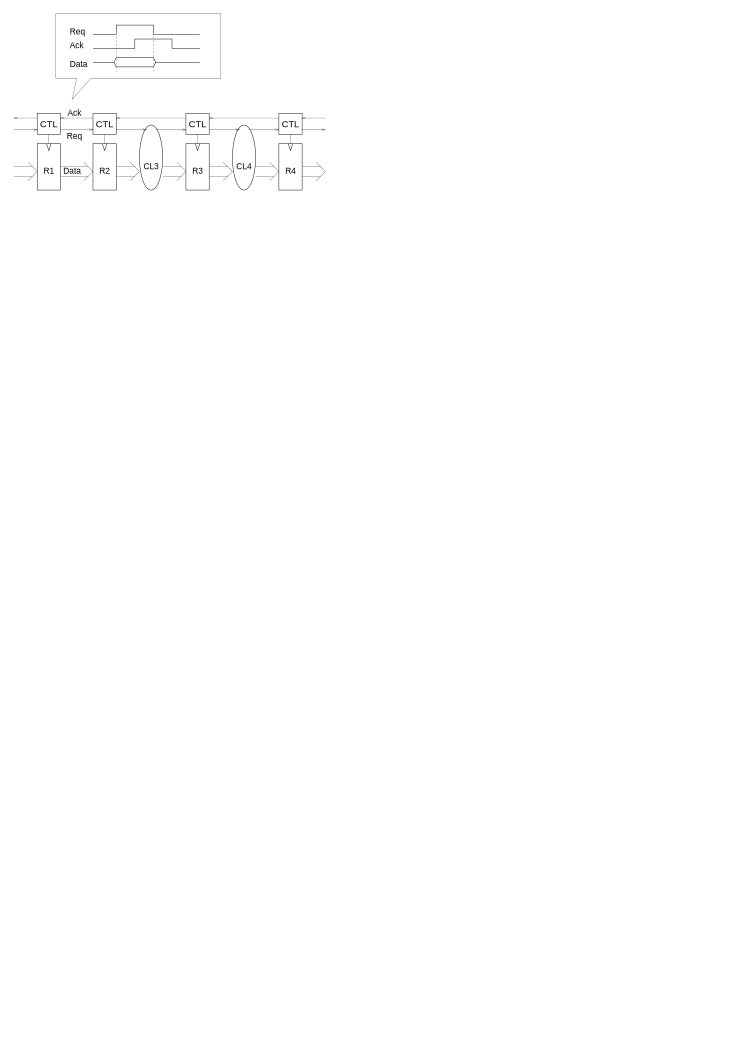
\includegraphics{handshake.pdf}
  \caption{A clockless pipeline implemented with handshaking ensuring
    data validity. The channels are bundled data four phase push
    channels. Figure from \cite{sparso}.}
  \label{fig:handshake}
\end{figure}

To connect and synchronize blocks in a clockless circuits, a form of
handshaking is usually employed, often as as a request-acknowledge
protocol shown in figure~\ref{fig:handshake}. The handshaking provides
a local clock for the storage elements, usually latches or C-elements.

There are multiple ways to implement handshaking. Some high level
synthesis tools, introduced in section~\ref{sec:tools}, allows the
designer to choose and evaluate multiple implementation styles. The
Tangram/Haste synthesis tool allows handshake circuits to be
implemented as clocked circuits, making verification on regular FPGAs
\nomenclature{FPGA}{Field-Programmable Gate-Array} possible.

\subsection{Encodings}

Clocked digital circuits often use regular binary encoding where one
wire corresponds to one bit, a high voltage corresponds to a 1 and a
low voltage to a 0. While this encoding is possible with clockless
circuits, it has the drawback of not indicating completion. Other
encodings, discussed below, can also provide completion detection, an
important property of a QDI design. Choice of encodings has also been
shown to have significant impact on power.
 
\begin{figure}[htbp]
  \centering
  \includegraphics{bundled.pdf}
  \caption{An abstract view of a channel with bundled data, and two
    different protocols for data validity. Figure from \cite{sparso}.}
  \label{fig:bundled}
\end{figure}

When using bundled data, values are represented by conventional
boolean levels, and the handshaking is implemented by bundling request
and acknowledge signals with data as shown in
figure~\ref{fig:bundled}~a). Bundled data is also refered to as single
rail, in contrast to e.g. dual rail encoding, as data is encoded as
ordinary binary data. Usually there is no way to determine wether
binary data from a combinatonal function is complete, delays matching
the combinational delay in the critical path have to be inserted in
the control path to maintain correct behaviour as shown in
figure~\ref{fig:bundeled_delay}.

\begin{table}
  \centering
  \begin{tabular}{|c|c|}
    \hline
    \emph{Electrical signal} & \emph{Interpretation} \\
    \hline
    0 0 & ``NULL''; no value \\
    0 1 & false, 0 \\
    1 0 & true, 1 \\
    1 1 & invalid \\
    \hline
  \end{tabular}
  \label{tab:dr}
  \caption{Dual rail representation of a boolean value.}
\end{table}

If the signal is encoded into a representation using two wires per
bit, one for each value; logic 1 (true) and logic 0 (false), it is
possible to distinguish successive values by seperating them with an
``empty'' value, also referred to as a ``NULL''. This encoding is
referred to as ``dual rail'' encoding, and is summarized in
table~\ref{tab:dr}.

\begin{figure}[htbp]
  \centering
  \includegraphics{drgate.pdf}
  \caption{a) A dual rail inverter. b) A strongly indicating dual rail
    and-gate, and c) the simulated and-gate. Note that the output is
    not showing a value until both inputs does, and that the value is
    held until \emph{both} imputs are returned to ``NULL''.}
  \label{fig:drgate}
\end{figure}

When implementing combinational functions for dual rail encoding, they
are typically split into two functions analogous to the pull up and
pull down networks in CMOS; one to compute the logic 0 or false value,
and one to compute the logic 1 or true value. A dual rail gate
implementation illustrating this is shown in figure~\ref{fig:drgate},
where one C-element is used to calculate a 1, and the other gates are
used to calculate a 0. Dual rail gates can often be less complex than
the example, by combining and optimizing the gates. While the and-gate
implementation shown in figure~\ref{fig:drgate} is state-holding, and
holds a calculated value until all (both) inputs returns to NULL, not
all gates need to have such complicated implementations. Usually, the
double area is needed to implement a dual-rail circuit over that of
single-rail.

A more generalized method for encoding, is N of M encodings, where
dual rail is 1 of 2 encoding. All these encodings are constant-weight
(N) encodings, meaning that a complete signal has a certain hamming
weight, that is the count of electrical ones on a complete signal. In
\cite[chapter 9]{nullconv}, multiple of these encodings are surveyed
with regards to required resources (i.e. area) for wires and logic,
and power. An ALU for 1 of 4 encoding are shown to have good
characteristics in terms of power, area and performance, compared to
the dual rail encoding.

\subsection{Protocol}

When using handshake protocols, the handshake can be done in four or
two phases as shown in figure~\ref{fig:bundled}~b) and c). The four
phase protocol is also referred to as return to zero (RTZ). The two
phase protocol makes better use of the bandwith over the wires, but
usually the four phase protocol is preferred, as it allows for a
simpler implementation consuming less area.

In figure~\ref{fig:bundled}~a), a \emph{push} channel is shown. This
means that the data source initiates the handshake with the request
signal, as opposed to when the receiver inititates it. A channel where
the receiver initiates the handshake is referred to as a \emph{pull}
channel.

\begin{figure}[htbp]
  \centering
  \includegraphics{compdet.pdf}
  \caption{A memory element for dual-rail implementations with
    completion detection. Figure from \cite[pp. 21]{sparso}.}
  \label{fig:compdet}
\end{figure}

In the case of QDI (e.g. dual-rail) encodings, completion detection
provides either the request or acknowledge signal. Completion is
detected by counting the number of electrical ones, as shown in
figure~\ref{fig:compdet}, providing either a request signal in the
case of a push channel, or an acknowledge signal in the case of a pull
channel. The completion detector in figure~\ref{fig:compdet} provides
the request signal, and is therefore the receiver in a push channel.

Using dual rail encoding usually also implies using the four phase
protocol\footnote{For the sake of completeness, two phase protocol is
  possible with level-encoded two phase dual-rail (LEDR)\cite{ledr},
  but it is considered impractical for other uses than on long wires
  on chip.}  (figure~\ref{fig:bundled}~b)), as the combinational
circuits must return to the NULL state between values to distinguish
successive values on the channel. Care must therefore not only be
taken to avoid hazards on NULL-to-value transitions, but also on the
return-to-NULL transitions.

Hazards are avoided by adding redundant gates XXX

\subsection{Testing}

When producing integrated circuits, it is vital to ensure that the
defective ICs are removed from the production line as soon as
possible. Multiple defects can occur during modern fabrication that
can render ICs unusable or limit lifetime.

To determine which chips that are OK and not, testing must be
performed. Testing methods was divided into two categories by
\cite{xxx}: Functional testing, and structural testing.

In functional testing, the circuit is tested in its normal operation
mode, and no modifications to the circuit is needed. However, without
good knowledge of the underlying logic of a circuit under test, only
exhaustive testing can guarantee that the circuit will function for
all possible inputs. For e.g. a 32-bit adder, this means that $2^{64}
\approx 10^{19}$ vectors must be tested, which will, at an
unreasonable high test frequency of \unit{1}{\giga \hertz}, take
approximatly \unit{10^{10}}{\second}, or 317 years to perform, leaving
functional testing unreasonable for this circuit.

Another form for functional testing, built in self test
(BIST\nomenclature{BIST}{Built-In Self Test}), utilizes e.g. an on
chip processor to test the functionality present on the chip, and can
also be used to determine the maximum safe operating speed of the
chip, as this test runs ``at speed''. An example of BIST is the
testing of RAM by writing and verifying all bits accessible. BIST is
possible to implement both on clocked and clockless circuits.

Whith structural testing, a \emph{fault model} is choosen to give a
simplified, but reasonable model of defects that can occur. Based on
the fault mode, test patterns are generated to cover the maximum
number of faults, that is inputs that will yield a wrong output in the
presence of a fault.

To design-for-test (DfT\nomenclature{DfT}{Design-for-Test}) is to
design hardware with modifications to make it more testable. More
complicated circuits thant the mentioned 32 bit adder where inputs can
be controlled, and outputs observed, are circuits where inputs are
driven by e.g. internal registers, and where the outputs are not
directly observable. In such circuits, either aribtrarly long
sequences must be applied to steer and observe the registers, or test
points must be inserted.

Whith clocked circuits, such test points are usually implemented by
connecting multiplexers to registers, choosing whether the circuit
should operate in the normal mode, or that the regusters should be
connected in series, making a scan-chain. Scan-chains are
shift-registers that makes it possible to control and observe all the
scan-enabled registers. Scan-chains also allows single-stepping the
circuit, and by stopping the clock (and traditionally the entire
circuit), $I_{DDQ}$ tests can be performed to find shorts in the
circuit.

\begin{figure}[htbp]
  \centering
  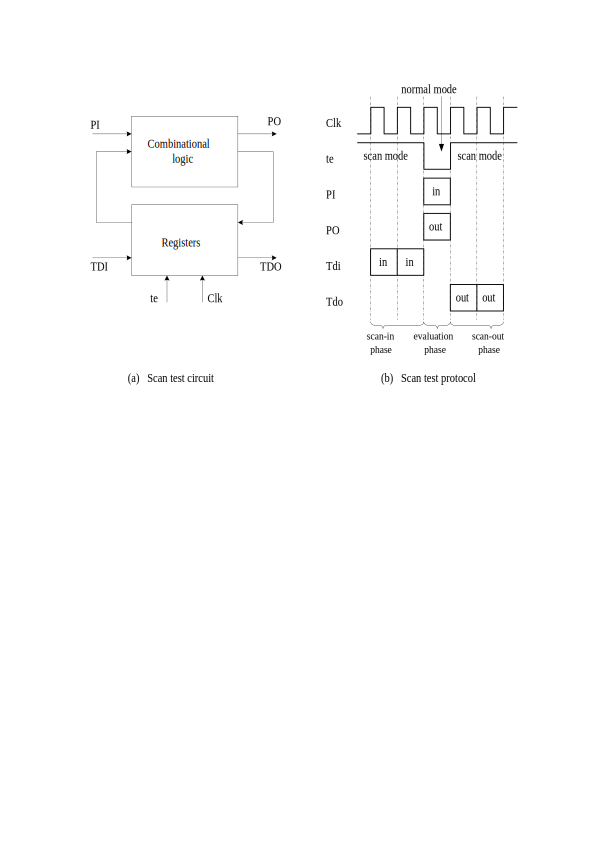
\includegraphics{scanint.pdf}
  \caption{a) A synchronous scan-interface, and b) protocol. Figure
    from \cite[pp. 11]{fullscan}.}
  \label{fig:scanint}
\end{figure}

Figure~\ref{fig:scanint} shows a typical scan-interface. This is
fairly standard, and equipment to interface with it is fairly
standard, and considered an industry standard. Therefore, it is
a good idea to implement the same interface for testing for clockless
circuit, to make it a more attractive method of producing circuits.

In \cite[pp. 27-28]{sparso} testing of clockless circuits is briefly
discussed, noting that the indication-principle will cause a circuit
with a stuck-at fault to deadlock. In \cite[pp. 26]{fullscan}, this is
referred to as the ``acknowledge property'', and it is noted that this
only holds for the practical unusefull class of delay-insensitive
circuits. In the more appliciable quasi delay insensitive kind of
circuits, isochronic forks can extend faults to not only cause a
circuit to deadlock, but also lead to a misbehaving circuit. XXX need
figure and cite.  Furthermore, \cite{fullscan} provides methods for
implementing a synchronous scan-interface to clockless circuits are
introduced and tested.

\subsection{Initialization and reset}

A clocked circuit is usually started by asserting a reset signal to
put it in a defined state,and then releasing the reset signal to let
the circuit start operating. The reset signal is either said to be
synchronous or asynchronous with regards to the global clock. A
synchronous reset signal must, as other signals, arrive within the
setup and hold times of the flip flops. An asynchronous reset must be
released simultainously across the whole circuit, a problem which is
as hard as distributing a global clock.

Not all parts of a circuit usually needs to be set in a known state
for a circuit to operate correctly. E.g. a circuit that receives some
input into registers, processes the data, and then outputs the
results, need not to reset the data-registers as they will be
overwritten before the register content is used in the calculations.

Clockless circuits also need initialization, but based on the
read-after-write principle illustrated above, in principle only the
top-most control circuit needs initialization, which then initializes
sub circuits with handshaking when needed. This method of
initialization is generally used in handshake circuits described
in~\ref{sec:tools} on page~\pageref{par:init}.


\clearpage
\newpage
\section{Survey of available tools}

xxx

\clearpage
\newpage


\section{The Advanced Encryption Standard (AES)}

On September 12, 1997, the United States' National Institute of
Standards and Technology (NIST) announced an open competition to
develop a new symmetric-key block cipher algorithm to replace the
ageing DES (Data Encryption Standard). The demands was that the AES
should be an unclassified, public, and royalty-free symmetric-key
encryption algorithm supporting block sizes of 128-bits, key sizes of
128-, 192- and 256-bits.

On October 2, 2000, NIST announced that it had selected
Rijandael~\cite{rijandael}, designed by two Belgium cryptographers:
Daemen and Rijmen, as the AES.

%As of today, multiple processors include native support for
%acceleration of AES-specific operations. NIST has also called for the
%development of a new hash-function, and 4 of 14 of the remaining
%candidates rely on native AES-acceleration to acheive performance.

\subsection{Overview of the algorithm}

Rijandael is a symmetric-key block-cipher algorithm. This means that
encryption is defined as $c \leftarrow E_k(m)$, and decryption as $m
\leftarrow D_k(c)$, given a key $k$, a message $m$ and a ciphertext
$c$. Rijandael supports variable block and key sizes, but I will
confine the description and implementation to block and key size to
128~bits. This will not cause a big loss of generality to the working
principle. I will also limit the implementation to encryption-only.

The Rijandael cipher segments a 128-bit message into 16 bytes,
represented by a $4 \times 4$ matrix:

\begin{equation}
  m = \begin{pmatrix}
    m_0 & m_4 & m_8 & m_{12} \\
    m_1 & m_5 & m_9 & m_{13} \\
    m_2 & m_6 & m_{10} & m_{14} \\
    m_3 & m_7 & m_{11} & m_{15}
    \end{pmatrix}
\end{equation}

This is referred to as the $State$ througout the algorithm, and it
is permutated 10 rounds in the algorithm. For larger key sizes, the
number of rounds should be increased. A round is composed of four
transformations described below:

\begin{eqnarray}
&Round&(State, RoundKey) \{\\
  & &SubBytes (State)\\
  & &ShiftRows (State)\\
  & &MixColumns (State)\\
  & &AddRoundKey (State, RoundKey)\\
&\}&
\end{eqnarray}

The final round, $FinalRound$, is slightly different: it excludes the
MixColumns stage. $RoundKey$ is derived from the key by the key
expansion scheme also described below. For decrypting, given the
correct key, there exists inverse functions for each round.

The Rijandael cipher work in a finite field. The field is realized as
all polynomials modulo the irreducivle polynomial $f(x) = x^8 + x^4 +
x^3 + x + 1$ over $\mathbb{F}_2$. This is called the ``Rijandael
field'', and $\mathbb{F}_{w^8}$ is often used to denote the field with
256 element. Each element can also be represented as a 8-bit byte. All
operations on elements in this field results in an element within the
field. The field supports addition and multiplication between two
field elements.

The $SubBytes$ routing subtitutes all bytes using the following formula:

$y = A x^{-1} + b$, where $
  A =
  \begin{pmatrix}
    1 & 0 & 0 & 0 & 1 & 1 & 1 & 1 \\
    1 & 1 & 0 & 0 & 0 & 1 & 1 & 1 \\
    1 & 1 & 1 & 0 & 0 & 0 & 1 & 1 \\
    1 & 1 & 1 & 1 & 0 & 0 & 0 & 1 \\
    1 & 1 & 1 & 1 & 1 & 0 & 0 & 0 \\
    0 & 1 & 1 & 1 & 1 & 1 & 0 & 0 \\
    0 & 0 & 1 & 1 & 1 & 1 & 1 & 0 \\
    0 & 0 & 0 & 1 & 1 & 1 & 1 & 1
  \end{pmatrix}$ and $
  b = 
  \begin{pmatrix}
    1\\1\\0\\0\\0\\1\\1\\0
  \end{pmatrix}$.
That is, inversion in the finite galois-field, followed by a short
final and linear transformation.

$ShiftRows$ is a permutation of the order of the bytes in the state:
\begin{equation}
  \begin{pmatrix}
    s_0 & s_4 & s_8    & s_{12} \\
    s_1 & s_5 & s_9    & s_{13} \\
    s_2 & s_6 & s_{10} & s_{14} \\
    s_3 & s_7 & s_{11} & s_{15}
  \end{pmatrix} 
  \rightarrow
  \begin{pmatrix}
    s_0    & s_4    & s_8    & s_{12} \\
    s_{13} & s_1    & s_5    & s_9 \\
    s_{10} & s_{14} & s_2    & s_6 \\
    s_7    & s_{11} & s_{15} & s_3    
    \end{pmatrix}
\end{equation}.
In VLSI circuits, this is easily implemented as wiring.

The $MixColumn$ procedure scrambles all the columns in the state,
given as $
\begin{pmatrix}
  s_0\\s_1\\s_2\\s_3
\end{pmatrix}$, 
by multiplying them with the matrix $
\begin{pmatrix}
  2 & 3 & 1 & 1 \\
  1 & 2 & 3 & 1 \\
  1 & 1 & 2 & 3 \\
  3 & 1 & 1 & 2
\end{pmatrix}$ 
in the galois field. Multiplication, $q(x)=a(x)b(x)$, can be performed
by generating eight partial products $P_i(x) = a(x) x^i$ and then add
them as $q(x) = \sum_{i=0}^{7} P_i b_i$, according to the bits $b_i$
in $b(x)$.

$AddRoundKey$ performs simple addition of the expanded key and the
state in the galois field. This addition can be implemented by simple
xor. The expanded key, derived from the input key, is calculated by
operations similar to the round function, and needs 4 bytes of
$SubBytes$ transformation as well.

\subsection{Implementation details for VLSI implementation}

\subsubsection{$SubBytes$ implementations}

Usually, the $SubBytes$ routine and its inverse is implemented with a
table lookup with 256 entries. In hardware, this means some kind of a
ROM, with an unbreakable latency and the inherent impossibility for
pipelining. In \cite{csbox} a method is described for decomposing the
$2^8$ fields into smaller $2^4$ fields for calculating the inverse
combinationally.

\subsubsection{Word width}

\subsubsection{Resource sharing}


\subsubsection{Pipelining and mode of operation}

While it is possible to pipeline the $Round$ procedure by itself, and
even $SubBytes$ itself when implemented combinationally as in
\cite{csbox}, it can also be beneficial to unroll multiple $Round$s in
series as shown in figure~\ref{fig:unroll}. I will here describe 3
modes of operation to illustrate when unrolling can be beneficial.

When encrypting a plaintext with a length over 128 bits, the most
straightforward way is to split the plaintext into 128-bit blocks and
encrypt them individually. This is called the electronic codebook mode
of operation, or ECB. As the blocks can be encrypted and decrypted
independently, this method allows pipelining with unrolled
$Round$s. However, as the AES-algorithm deterministicly yields the
same output given the same input (key and data), it allows an attacker
to guess the ciphertext by trial-and-error. Figure~\ref{fig:ecbpict}
shows how ECB reveals data-patterns from the plaintext.

The output feedback (OFB) mode of operation, described in
figure~\ref{fig:ofb}, while not suffering from the same weakness as
the ECB mode, does not benefit from unrolling, as the preceeding
ciphertext is needed to encrypt the current plaintext. The OFB mode
generates a pseudo random (but unguessable, not given the key) string
that is XORed with the plaintext to encrypt, similar to the Vernam
one-time-pad cipher \cite{vernam}.

The only mode of operation considered secure, to my knowledge, that
benefit from loop unrolling, is the counter (CTR) mode. In this mode,
similar to the OFB mode, a pseudorandom string is generated simpy by
encrypting an integer corresponding to the current block number, that
is $c_i \leftarrow m_i \oplus E_k(i)$, and similarily $m_i \leftarrow
c_i \oplus E_k(i)$. Whithout feedback, the CTR mode allows random
access during encryption and decryption (for e.g. full disk
encryption), and blocks can be processed in paralell.


\clearpage
\newpage

\section{Implementation of clockless AES}

xxx

\clearpage
\newpage
\section{Results and Discussion}

The emphasis of this project was not the AES module itself, but the
workflow outlined for specifying behaviour at a high level, and
obtaining a netlist correctly implementing the specified
behaviour.

\begin{table}[h]
  \centering
  \begin{tabular}{|c|c|}
    \hline
    \emph{Component}  & \emph{Count} \\ \hline
    AND2 & 8493 \\
    AND3 & 2 \\
    NAND2 & 501 \\
    NAND3 & 146 \\
    OR2 & 3982 \\
    OR3 & 39 \\
    NOR2 & 785 \\ 
    NOR3 & 1517 \\
    BUFF & 4131 \\
    INV & 560 \\
    AO22 & 692 \\
    AO222 & 8 \\
    C2 & 2609 \\
    C2R & 1093 \\
    C3  & 2130 \\
    AC2 & 0 \\
    \hline
  \end{tabular}
  \caption{Resource usage in terms of gates listed in
    figure~\ref{fig:teaklib} on page~\pageref{fig:teaklib}}
  \label{tab:res}
\end{table}

The Verilog netlist generated by Teak from the Balsa sourceode
contained 65421 lines. This also includes the test-bench enclosure,
inputting one key and plaintext, and printing the
ciphertext. Table~\ref{tab:res} summarizes the resource usage of the
Teak circuit, with the primitives illustrated in
figure~\ref{fig:teaklib} on page~\pageref{fig:teaklib}.

The performance was not measured, as this was a non-trivial procedure
with the choosen verilog simulator, which also prooved itself quite
unstable given the large verilog netlist. The litterature suggests
that my choices would yield a poorly performing circuit, as Teak has
been shown to currently perform worse than Balsa, which in turn
performs worse than conventional clocked circuits.

However, clockless circuits have other properties than clocked
circuits, which can be important for applications where performance is
not the primary objective. Low power is no longer considered a niche,
and as shown in \cite{claes}, clockless circuits can have good
characteristics with for secure implemetation of crypto algorithms.

It is also interesting how much effort that went into producing a
working AES module. I did not keep track of how many hours that went
into learning the Balsa language, or to write the AES, but after
understanding the basic handshake mechanisms, writing working Balsa
programs was quite straighforward. CSP languages, as noted in
\cite{taylor}, allows specifications to be expressed in way that is
similar to programmers accustomed to imperative programming languages,
such as C, lowering the threshold for doing hardware design, ``even
for novices''. While specifications written in CSP style languages
such as Balsa and Tangram are not guaranteed to be efficiently
implemented, tools such as visual simulators allows the designer to
gain a better understanding of how the design performs, find
bottlenecks and to optimize the sourcecode when required.

While low area and high performance are often cited goals for a
digital circuit specification, the time consumed by engineers to
design and verify a circuit is also important. If a design meets the
required constraints, e.g. it meet its realtime deadlies, and the
design fits on a specified FPGA, no further optimizations should be
required.

While I was able to develop an AES with the available tools, I
encountered bugs on many occasions, which I sometimes was not able to
work around. The most important problem was a compiler bug in Balsa
3.5.1, which prevented compilation of my AES module. I was later
supplied with the newest Balsa 4.0 which was able to generate
handshake circuits in the Breeze-format, but not able to further
generate netlists. While this illustrates that the choosen tools are
currently a bit immature, they are under development, and are expected
to improve.


\clearpage
\newpage
\section{Conclusion}

In this project, methods for creating circuits without clocks have
been researched, and a clockless AES-module have been implemented to a
netlist comprising of primitive gates, using the Balsa language and
Teak synthesis system.

\subsection{Further work}

Insertion of scan chains

Power estimation.

Technology mapping.

Place \& route

Optimize performance.

\begin{quotation}
  ``I regard programs as specific instances of mechanisms, and I wanted
  to express, at least once, my strong feeling that many of my
  considerations concerning software are, mutatis mutandis, just as
  relevant for hardware design''

  --Edsger W. Dijkstra
\end{quotation}



\clearpage
\newpage
\appendix

\section{Sourcecode}

\lstset{ %
basicstyle=\footnotesize,       % the size of the fonts that are used for the code
numbers=left,                   % where to put the line-numbers
numberstyle=\footnotesize,      % the size of the fonts that are used for the line-numbers
stepnumber=1,                   % the step between two line-numbers. If it's 1 each line will be numbered
numbersep=5pt,                  % how far the line-numbers are from the code
showspaces=false,               % show spaces adding particular underscores
showstringspaces=false,         % underline spaces within strings
showtabs=false,                 % show tabs within strings adding particular underscores
frame=single,                % adds a frame around the code
tabsize=3,                % sets default tabsize to 2 spaces
captionpos=b,                   % sets the caption-position to bottom
breaklines=true,                % sets automatic line breaking
breakatwhitespace=false,        % sets if automatic breaks should only happen at whitespace
escapeinside={\%*}{*)}          % if you want to add a comment within your code
}


\subsection{Test fixture, test-simple.balsa}
\lstinputlisting{naive-AES-balsa/test-simple.balsa}

\subsection{aes.balsa}
\lstinputlisting{naive-AES-balsa/aes.balsa}

\subsection{sbox.balsa}
\lstinputlisting{naive-AES-balsa/sbox.balsa}

\subsubsection{affine.balsa}
\lstinputlisting{naive-AES-balsa/affine.balsa}

\subsubsection{inversion.balsa}
\lstinputlisting{naive-AES-balsa/inversion.balsa}

\subsubsection{gf4.balsa}
\lstinputlisting{naive-AES-balsa/gf4.balsa}


\subsection{mixcolumn.balsa}
\lstinputlisting{naive-AES-balsa/mixcolumn.balsa}

\subsection{gfdouble.balsa}
\lstinputlisting{naive-AES-balsa/gfdouble.balsa}

\clearpage
\newpage

\section{Software}

XXX: Software

\begin{itemize}
  \item Balsa version 3.5.1
  \item Balsa version 4.0, supplied on XXX
  \item Teak, supplied XXX
  \item CVer verilog simulator version 2.12a-1 
\end{itemize}


%\input{fremdriftsplan}
%\clearpage
%\newpage

\clearpage
\newpage
\label{ssec:littref}

\bibliographystyle{IEEEtran}

\bibliography{boker} 


\end{document}

